\Titular*%
{Viaxeiros espaciais. Oda á Voyager 1}%
{Celia Álvarez Álvarez}%
{historia}%
{De como a Voyager 1 partiu dende a Terra ata o espazo profundo.}%

\begin{refsection}
\begin{multicols}{2}

\subsection*{\textit{Na beira do océano cósmico}.}

<<\textit{A superficie da Terra é a beira do océano cósmico. Dela aprendemos a
maior parte do que sabemos. Recentemente metémonos un pouco no mar, vadeando o
xusto para mollarnos os dedos dos pés ou, como moito, para que a auga nos
chegase aos nocellos. A auga parece convidarnos a continuar. O océano chámanos.
Hai unha parte de nós que sabe que vimos de alí. Desexamos volver. Non creo que
estas aspiracións sexan irreverentes, mesmo se poden desagradar aos deuses,
sexan cales foren os posibles deuses.}>> 

%\vspace*{-1mm}
%\begin{flushright}
%Carl Sagan, \textit{Cosmos} (adaptación).
%\end{flushright}
\hfill Carl Sagan, \textit{Cosmos} (adaptación). \\

A misión de investigación espacial Voyager, fundada pola NASA, está constituída
por dúas sondas interestelares irmás: a Voyager 1 e a Voyager 2.

Durante a travesía do Voyager 1 tiveron lugar investigacións exploratorias dos
sistemas planetarios xoviano e saturniano e do medio interplanetario. O estudo
abrangueu a mellora na nosa comprensión das dinámicas atmosféricas de Xúpiter e
Saturno, dos seus campos gravitatorios, das súas magnetosferas, das
interaccións dos satélites con todos estes factores, das composicións
atmosféricas e superficiais de satélites como Titán ou os catro satélites
galileanos: Io, Europa, Ganímedes e Calisto, da Gran Mancha Vermella de Xúpiter
ou dos aneis de Saturno.

Para iso, a Voyager 1 levou a bordo instrumentos para desenvolver once
investigacións científicas, entre elas: o \textit{Imaging Science System}
(ISS), que permitiu capturar espectaculares imaxes do sistema solar; o
\textit{Infrared interferometer spectrometer and radiometer} (IRIS), que
permitiu obter perfís de enerxías e temperaturas; o \textit{Triaxial Fluxgate
Magnetometer} (MAG), que investiga os campos magnéticos de planetas e do espazo
interplanetario; o \textit{Low Energy Charged Particle Instrument} (LECP), que
mide propiedades de electróns ou ións de plasma detectados; ou o \textit{Plasma
Wave Subsystem} (PWS), que tamén se utiliza no estudo de magnetosferas e da
interacción local onda-partícula. Actualmente só o MAG, o LECP e o PWS se
atopan activos.

A sonda obtén a súa enerxía de tres xeradores termoeléctricos de radioisótopos,
que funcionan grazas á desintegración do óxido de plutonio. Estes xeradores
converten calor producido na desintegración radioactiva en enerxía eléctrica. A
potencia dos xeradores diminúe co tempo debido á semivida do combustible e á
degradación dos termopares, polos cales se converte enerxía térmica en
eléctrica mediante o efecto Seebeck. Durante a navegación utilízanse sinais do
rastreador solar e estelar para conservar a antena de radio do Voyager
orientada cara á Terra activando pequenos propulsores do sistema de propulsión
da Voyager.

\subsection*{Viaxe. Navegando polo sistema solar.}

Dúas naves Voyager ían ser lanzadas durante a ventá % igual hai que darlle
voltas a esa expresión dun mes que comezaba a finais de agosto de 1977,
coincidindo cun aliñamento especial  dos planetas exteriores que permitiría o
uso dos seus campos gravitacionais para cambiar a velocidade e dirección da
sonda e así facilitar a súa viaxe dun cara ao seguinte.

Orixinalmente programada para partir doce días despois da Voyager 2, a Voyager
1 tivo o seu despegue a bordo do vehículo de lanzamento \textit{Titan IIE} tras
ser aprazado en dúas ocasións para previr os problemas que sucederan tralo
lanzamento da Voyager 2. A partida definitiva da sonda sucedeu o 5 de setembro
de 1977 ás 12:56:00 UTC dende a Estación da Forza Espacial de Cabo Cañaveral
(Florida, EEUU), cun lanzamento impecable e preciso. O 6 de setembro, un día
despois da partida, a Voyager despediuse da Terra e da Lúa mandando a súa
primeira foto do noso hogar e o seu único satélite.

Pouco despois da saída da Voyager da órbita terreste todos os instrumentos
científicos acendérose para aproveitar as características que se comparten a
Terra e a Lúa con Xúpiter, Saturno e os seus satélites; realizáronse
observacións útiles para a súa calibración. Trinta días despois do lanzamento
comeza oficialmente a fase de cruceiro ata o encontro con Xúpiter. Os
instrumentos para o estudo de campos e partículas na Voyager investigaron
durante este tempo a rexión interplanetaria Terra-Xúpiter. A Voyager 1 adiantou
á Voyager 2 tras adentrarse no cinto de asteroides.

Ointenta días antes do encontro con Xúpiter comezaron as observacións do
planeta e dos satélites galileanos. A esta distancia a cámara ISS da Voyager
pode obter unha resolución comparable ou mellor que a alcanzable na Terra. A
Voyager 1 alcanza o seu achegamento máis próximo a Xúpiter o 5 de marzo de
1979: a sonda sobrevoou o satélite xoviano Amaltea, descubrindo a súa forma
alongada; seis horas despois, a Voyager atoparase a uns 350.000 km do centro de
masa de Xúpiter para logo sobrevoar Io, Europa, Ganímedes e Calisto.

\begin{center}
    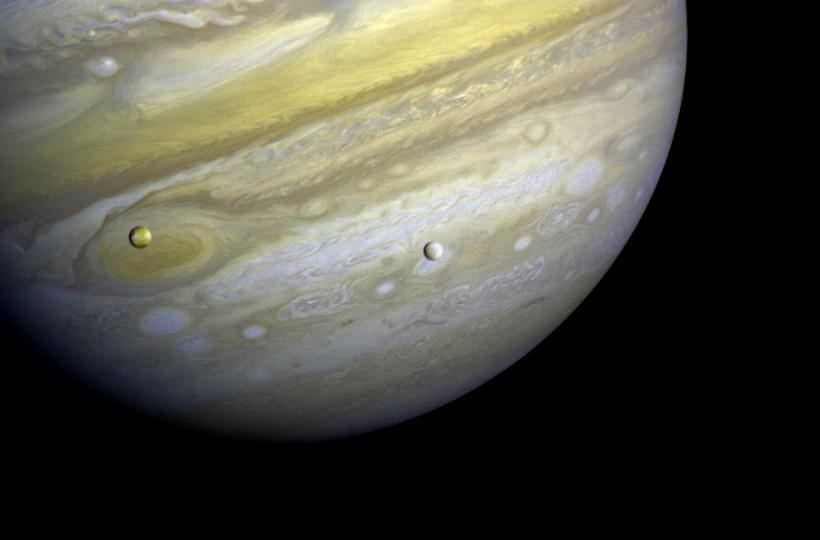
\includegraphics[width=0.9\linewidth]{revistas/002/imaxes/jupiter.jpg}
    \captionof{figure}{Xúpiter cos satélites Io (esquerda) e Europa.}
\end{center}

Descubríronse o sistema xoviano de aneis e dúas lúas, Thebe e Metis, detectouse
o primeiro relámpago nun mundo máis aló da Terra, desvélase que a Gran Mancha
Vermella se trata dunha grandísima tormenta que recorda a un ciclón e avístanse
en Io os primeiros volcáns activos fóra da Terra. A Voyager 1 comeza a súa
viaxe cara Saturno deixando ao redor de 180.000 fotografías do sistema xoviano,
incluíndo películas a cor das dinámicas das nubes xovianas.

\begin{center}
    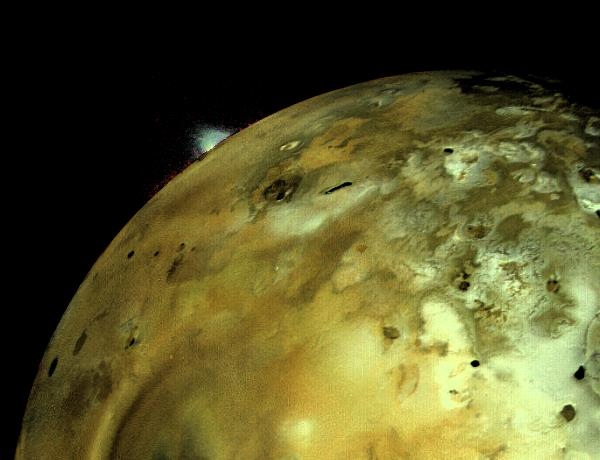
\includegraphics[width=0.8\linewidth]{revistas/002/imaxes/io.jpg}
    \captionof{figure}{Explosión do volcán Loki en Io.}
\end{center}

O 9 de novembro de 1980 sucede o encontro coa lúa máis grande de Saturno,
Titán, e co propio Saturno. Descúbrense Atlas, Prometeo e Pandora, tres
``pequenas'' lúas das máis de duascentas que actualmente se coñecen orbitando
este xigante gaseoso. As órbitas de Prometeo e Pandora ao redor dos aneis F de
Saturno confirman a teoría da existenca de ``satélites pastores'' que producen
ocos nos aneis e fixan gravitacionalmente os seus bordos. Recóllense vistas da
brillante superficie de Encélado e obsérvanse formas enigmáticas nos aneis de
Saturno que se pasarían a denominar radios, cuxa orixe non se comprende
completamente na actualidade.

\begin{center}
    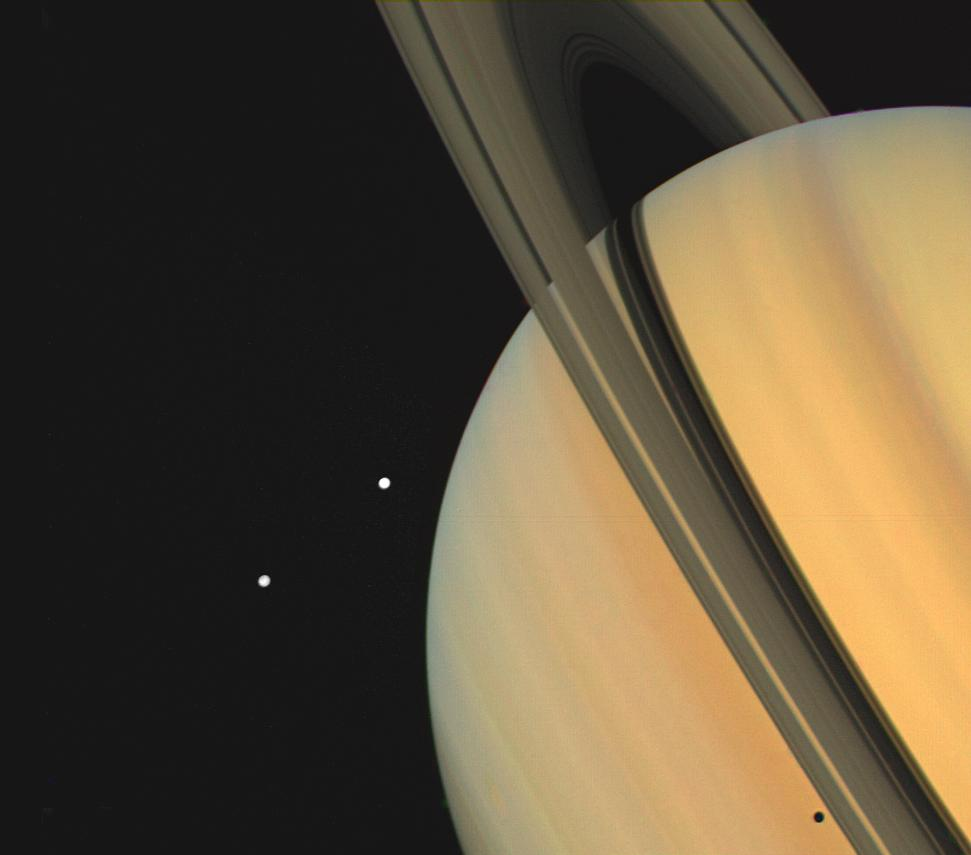
\includegraphics[width=0.8\linewidth]{revistas/002/imaxes/saturno.jpg}
    \captionof{figure}{Saturno con Tetis (arriba-dereita) e Dione. As
    sombras dos aneis e de Tetis proxéctanse nas nubes do planeta.}
\end{center}

\textbf{\textit{Life on Titan?}}

Titán é a segunda lúa máis grande do sistema solar tras Ganímedes e tamén é o
único lugar do sistema solar á parte do noso planeta en cuxa superficie se pode
atopar líquido estable en forma de ríos, lagos e mares. A súa densa atmosfera
neboenta e dourada está composta principalmente por nitróxeno e pequenas
cantidades de metano e etano. Os sinais de radio recibidos da Voyager 1
permitiron descubrir a existencia dunha superficie xeada en Titán, baixo a cal
existe un océano formado principalmente por auga que podería albergar formas de
vida, quizais a escala microscópica. Tan igual de plausible é que non haxa vida
en Titán. A misión \textit{Dragonfly} enviará unha aeronave rotatoria robótica,
será lanzada en xullo de 2028 e chegará a Titán en 2034.
\begin{center}
    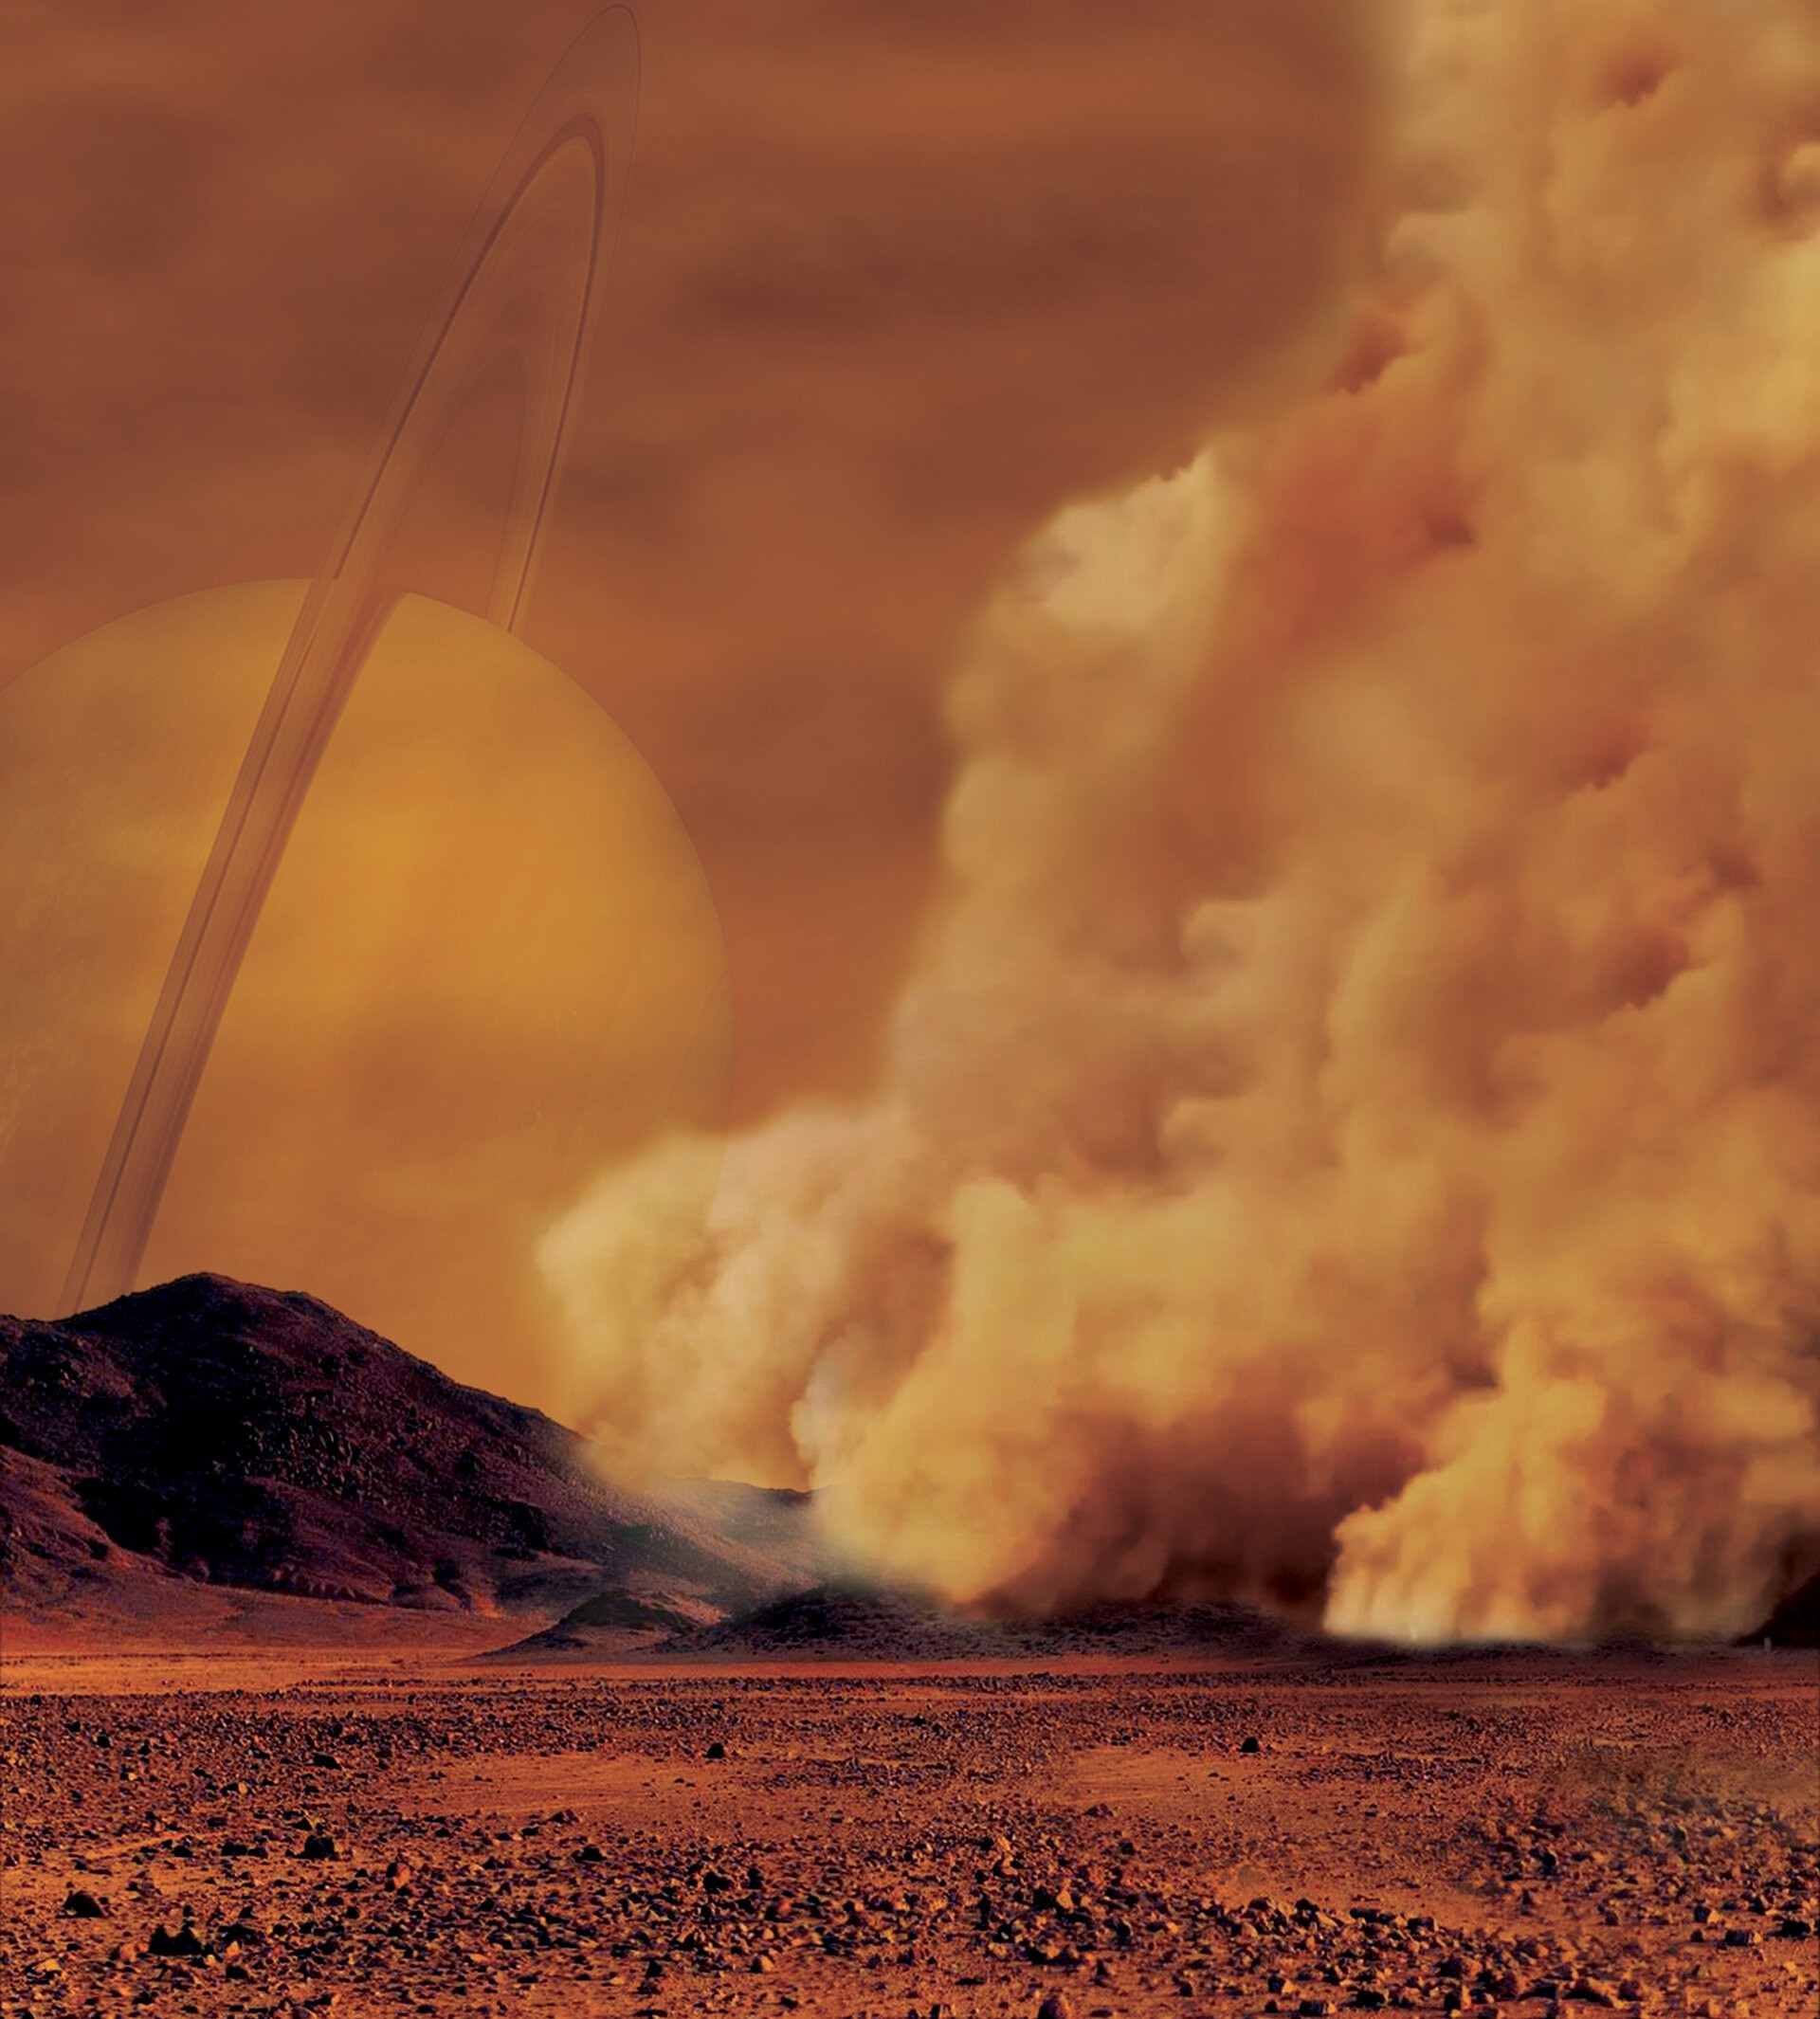
\includegraphics[width=0.6\linewidth]{revistas/002/imaxes/Dust_storm_on_Titan_pillars_corte.jpg}
    \captionof{figure}{Concepción artística de unha tormenta de pó en Titán con Saturno de fondo.}
\end{center}


\subsection*{Misión estendida. Saíndo do sistema solar.}



O 14 de novembro de 1980 comeza a misión extendida da Voyager 1. Recibindo un
impulso gravitacional, a sonda comeza a alonxarse do plano da eclíptica do
sistema solar e dez anos máis tarde, o 14 de febreiro de 1990, toma o
\textit{Retrato de familia} do sistema solar a petición do astrónomo Carl
Sagan: un mosaico composto de sesenta cadros individuais, as últimas imaxes
capturadas pola Voyager 1 antes de apagar a súa cámara ISS para sempre. A
Voyager 1 xa non voará preto de ningún outro obxecto astronómico en todo o
tempo no que durará o seu subministro enerxético polo que se prioriza o uso
deste en tarefas de recolección de datos do vento solar e do espazo
interestelar. A estas alturas, os febles sinais das sondas Voyager son
capturadas pola \textit{Deep Space Network} da NASA, con complexos en Goldstone
(California), Madrid e Canberra (Australia) que albergan grandes antenas de ata
setenta metros de diámetro.

\begin{center}
    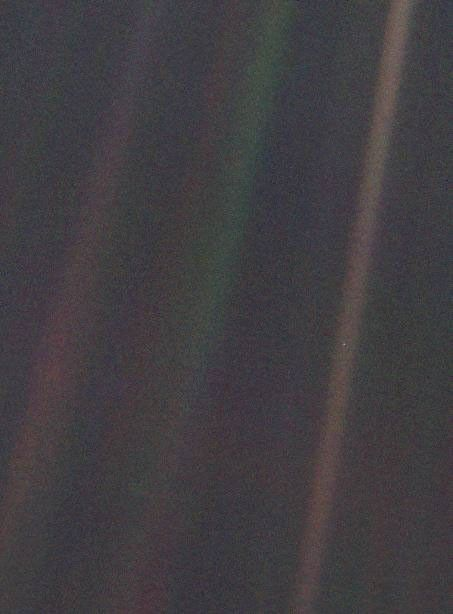
\includegraphics[width=0.6\linewidth]{revistas/002/imaxes/PaleBlueDot.jpg}
    \captionof{figure}{\textit{Pale Blue Dot}: imaxe da Terra tomada
        pola Voyager 1 para o \textit{Retrato de familia}. A Terra, vista
        a unha distancia de seis mil millóns de quilómetros, aparece coma
    un pequeno punto azulado na franxa vermella da dereita. }
\end{center}

O 17 de febreiro de 1998 a Voyager 1 sobrepasa a distancia do Pioneer 10 e
convírtese no obxecto feito polos humanos máis afastado da Terra, a unha
distancia de dez mil millóns de quilómetros. En decembro de 2004 a Voyager
alcanza a fronte de choque de terminación. Este é o límite coa última gran
rexión de dominio do vento solar, a heliosfera. O 25 de agosto de 2012 a
Voyager 1 convértese no primeiro obxecto humano no espazo interestelar
atravesando a fronteira da heliosfera, coñecida co nome de heliopausa. A
Voyager 1 ``escoitou'' os \textit{sons interestelares}. Vibracións do denso
plasma interestelar permitiron medir por primeira vez a densidade do medio
interestelar. Grazas á nosa tecnoloxía podemos transformar esas vibracións
eléctricas do plasma en zumbidos agudos e inquedantes que provocan calafríos.

Entre 2021 e 2024 a Voyager enfrentou varios desafíos relacionados coa
corrupción de datos e a súa transmisión á Terra, probablemente pola degradación
da aparataxe
% como dicía na nota, esta palabra non existe e en tal caso sería masculina
tras décadas de exposición á radiación espacial. Deste ano nunha década se
espera que a Voyager xa non dispoña de enerxía para alimentar ningún dos
instrumentos a bordo e perderemos o seu sinal para sempre.\\

\textbf{\textit{Message in a bottle.}}\\
Agárdase que a Voyager 1 entre na nube de Oort nuns trescentos anos. Esta é a
rexión de procedencia dos cometas de período longo e está situada a case un ano
luz do Sol e a un cuarto da distancia deste a \textit{Próxima Centauri}, a
estrela máis cercana ao sistema solar. A sonda tardará uns trinta mil anos en
saír dela sen rumbo particular cara a ningunha estrela. Estará destinada a
errar por toda a eternidade a través da Vía Láctea. Pasará moito tempo
viaxando, lonxe de ningunha illa estelar e portando o \textit{Golden Record}.
As Voyager son un primeiro grito cheo de esperanza que a humanidade lanzou
dende a beira do océano cósmico para darse a coñecer, unha mensaxe que di
\textit{hai alguén aí?}. \\

<<\textit{Quizais os rexistros nunca sexan interceptados. Quizais ninguén en
cinco mil millóns de anos os atope. Cinco mil millóns de anos é moito tempo. En
cinco mil millóns de anos, todos os seres humanos extinguiranse ou
evolucionarán noutros seres, ningún dos nosos artefactos sobrevivirá na Terra,
os continentes alteraranse ou destruiranse de forma irrecoñecible e a evolución
do Sol queimará a Terra ata convertela en} `crumble' \textit{ou a reducirá a un
remuíño de átomos.\\ Lonxe do fogar, intactas por estes acontecementos remotos,
as Voyagers, portadoras das lembranzas dun mundo que xa non existe, seguirán
voando.}>>

\hfill Carl Sagan, \textit{Pale Blue Dot} (adaptación).  

 % ao igual que antes hai que cambiar a cita


\nocite{oliver-berry.dmagmmvs_2019}
\nocite{sagan.c_2014}
\nocite{science_nasa_mission_voyager_timeline}
\nocite{photojournal_jpl_voyager_1}
\nocite{nasa_nssdc_gsfc}


\printbibliography

\end{multicols}
\end{refsection}
